\documentclass[12pt]{article}
\usepackage[english]{babel}
\usepackage{amsmath}
\usepackage{graphicx}
\usepackage{textcomp}
\usepackage{parskip}
\usepackage[colorinlistoftodos]{todonotes}
\usepackage{csquotes}
\usepackage{pifont}
\usepackage{float}
\newcommand\skiplines[1]{\vspace{#1\baselineskip}}
\usepackage{color}   %May be necessary if you want to color links
\usepackage{hyperref}
\hypersetup{
    colorlinks=true, %set true if you want colored links
    linktoc=all,     %set to all if you want both sections and subsections linked
    linkcolor=blue,  %choose some color if you want links to stand out
}

\usepackage[
backend=biber,
style=alphabetic,
sorting=ynt
]{biblatex}
\addbibresource{sample.bib}
\usepackage[a4paper,top=3cm,bottom=2cm,left=3cm,right=3cm,marginparwidth=1.75cm]{geometry}
\addbibresource{bibliography.bib}

\title{Usability Study Report of the GreenDrinks Website}
\author{Tomin Mattam \\Jade Fjestad \\                                                                                                               Jonathan Ballarin                                                                                                            	\\  Curtis Eck}

\begin{document}
University of Calgary \\
2500 University Drive N.W. \\
Calgary, Alberta \\
T2N 1N4 \\
 \newline
\today  \newline \\
Andrea Hanslip \\
Professor, Communications Studies 363   \\
2500 University Drive N.W. \\
Calgary, Alberta \\
T2N 1N4 \\

Dear Professor Andrea Hanslip: \\ \\
Re: Usability Study Report of the Green Drinks Website \\ \\
We have conducted a study to analyze the usability of the Green Drinks website. Our research methodology, findings, and recommendations can be found in the attached report: Usability Study Report of the Green Drinks Website.

We began our study with the COMS 363 course readings, to understand what well-done websites include. Once familiarized with the readings, we chose the criteria that we would focus on in the study. Then, each group member wrote a heuristic report on different aspects of websites. After, we created a usability web-based survey and got participants from our COMS 363 (L04) class. 

The findings of our study has indicated that the Green Drinks website needs to have some things changed to increase usability. The take-aways from the heuristic evaluations and the survey is that navigation, organization, and graphics need to improve. 

Our recommendations are based off of the heuristic evaluations and the survey. We broke the recommendations into four main groups and made many recommendations within each group. The four groups are to reduce the size of paragraphs to be more scannable, make the website more visually appealing, reformat the homepage to guide users to Find City, and add important information to the homepage.
\\ \\
Thank you for your time to read our report. \\ \\
Sincerely, \\ \\
Tomin Mattam                                                                                                              \\ Jade Fjestad                                                                                                              \\ Jonathan Ballarin                                                                                                           \\ and Curtis Eck
 
 

\begin{titlepage}

\newcommand{\HRule}{\rule{\linewidth}{0.5mm}} % Defines a new command for the horizontal lines, change thickness here

%----------------------------------------------------------------------------------------
%	LOGO SECTION
%----------------------------------------------------------------------------------------
\begin{center}

\includegraphics[width=5cm]{logo}
\end{center}
 % Include a department/university logo - this will require the graphicx package
 
%----------------------------------------------------------------------------------------

\center % Center everything on the page

%----------------------------------------------------------------------------------------
%	HEADING SECTIONS
%----------------------------------------------------------------------------------------

\textsc{\LARGE COMS 363 Final Report}\\[1.5cm] % Name of your university/college
\textsc{\Large University of Calgary}\\[0.5cm] % Major heading such as course name
\textsc{\large Department of Communications}\\[0.5cm] % Minor heading such as course title

%----------------------------------------------------------------------------------------
%	TITLE SECTION
%----------------------------------------------------------------------------------------
\makeatletter
\HRule \\[0.4cm]
{ \huge \bfseries \@title}\\[0.4cm] % Title of your document
\HRule \\[1.5cm]
 
%----------------------------------------------------------------------------------------
%	AUTHOR SECTION
%----------------------------------------------------------------------------------------

\begin{minipage}{0.4\textwidth}
\begin{flushleft} \large
\emph{Authors:}\\
\@author 
\end{flushleft}
\end{minipage}
~
\begin{minipage}{0.4\textwidth}
\begin{flushright} \large
\emph{Professor:} \\
Prof. Andrea Hanslip \\[1.2em] % Supervisor's Name

\end{flushright}
\end{minipage}\\[2cm]
\makeatother



{\large \today}\\[2cm] % Date, change the \today to a set date if you want to be precise

\vfill % Fill the rest of the page with whitespace

\end{titlepage}
\renewcommand{\abstractname}{Executive Summary}
\begin{abstract}
The purpose of this study was to determine the overall usability of the Green Drinks website. The website is a resource for those who frequently participate in Green Drink meetings. Therefore the website must be organized and usable for individuals to use the website. Green Drinks has a poor website design and needs many improvements. The criteria used to evaluate the website included:
\begin{itemize}
\item Strategy
\item Organization
\item Style
\end{itemize}
Heuristic evaluations were done by each group member on different aspects of websites. Group members researched effective ways to design a website for their aspect based on the criteria chosen. The Green Drinks website was compared to the aspects that were researched and the findings were written in the evaluation.
A web-based survey was used to ask participants, who were students from COMS 363 (L04), questions and to complete certain tasks on the Green Drinks website. The participants' feedback was taken into consideration when making recommendations.
The general conclusions found in this study was that there are many things that need to be changed to increase usability. The findings in the heuristic evaluations and the feedback from the survey are similar on what needs to change. From the information gathered we have many recommendations, we broke the recommendations up into four groups which include:
\begin{itemize}
\item Reduce the size of paragraphs to be more scannable.
\item Make the website more visually appealing.
\item Reformat the homepage to guide users to Find City.
\item Add important information to the homepage
\end{itemize}
\end{abstract}

\pagebreak

\setcounter{page}{1}
\thispagestyle{empty}
\tableofcontents 
	\newpage	
	{%
\let\oldnumberline\numberline%
\renewcommand{\numberline}{\figurename~\oldnumberline}%
\listoffigures%
}
\pagebreak
\setcounter{page}{1}


\pagebreak



\section{Introduction}
The purpose of this study was to determine the overall usability of the Green Drinks [1] website. The website is a resource for those who frequently participate in Green Drink meetings. Therefore the website must be organized and usable for individuals to use the website.

According to Lynch and Horton [2], visuals are an important aspect of a website. Without it, a website that is graphically uninteresting will demotivate its readers.This study looks at how organization and visuals impact a website, and how these aspects make a website more usable and available to the average user.

This report will talk about the following aspects of visuals and organization: Strategy, Organization of Information, and Style. These key aspects are necessary to any website design because it allows readers to use a website with ease. The Green Drinks website shows to be lacking in these aspects, making it a difficult website to use.
\section{Background}
Green Drinks was founded in 1990 by Edwin Datschefski, Paul Scott, Ian Grand and Yorick Benjamin [1]. The first Green Drinks gathering took place in London UK, consisting of friends and acquaintances. Over the years, Green Drinks has expanded across Europe. Eventually they had expanded overseas, making New York the first American state to join their organization. 

The organization’s goal is to allow those who share similar environmental interests to gather and discuss ecological ideas. The website’s purpose is to create these meetings and to spread the organization’s popularity to other people. Green Drinks [1] is a ‘self-organizing network’, meaning the meetings are managed through an organizer for each city. People who wish to attend these activities just approach the designated meeting area. 

One of the main aspects of this organization is that most of their interactions are in person. Since the website consists of no forums or online chats, all forms of communication are physical contact at the meetups. These meetings will usually occur once a month and on average consist of a hundred people.

\section{Objective}
The usability of the Green Drinks website was evaluated using the following criteria:

\begin{itemize}
\item Analyse the style and organization of information of the website
\item Critique website based on chosen criteria
\item Receive opinions from other users about the website
\item Create feedback and recommendations
\end{itemize}
\section{Research Methodology}
After reviewing the Green Drinks website we came up with three criteria to evaluate the website. Heuristic evaluations and a web-based survey were the research methods that were used for this study. These two methods were used to analyse the criteria to change the website to increase usability.

\section{Criteria}
The usability of the Green Drinks website was evaluated using the following criteria:
\begin{itemize}
\item Strategy
\item Organization
\item Style
\end{itemize}
\subsection{Strategy}
To investigate the strategy of the website, we looked to see if the goals of the website are clearly met. According to Lynch and Horton [2], the most important part of a website is to communicate the three main goals. For a website to be successful, it needs to effectively tell the users what the website is for. Additionally, the website should direct users to what to do. In the case of Green Drinks, users get information about their local meetups from the website. If the website cannot meet its goals, users are likely to never come back.



\subsection{Organization}
The organization is important so that users can effectively get the desired information from the site. As stated in Ewald [3], if users have any issues finding what they need from the resource, it has failed to effectively organize its content. The display on the site should be formatted in a way that is intuitive for the users to find what they need.
\subsection{Style}
The style of the website should convey to the user the quality of the organization. Sharpened Productions [4] suggests that a poorly styled website provides a bad first impression upon the user and can even turn them away. Today, with so many websites being built with WordPress (\url{https://wordpress.com/}) and GoDaddy (\url{https://ca.godaddy.com/}), the website standard aesthetic has risen. It is more obvious when a website looks old and unmaintained. An unmaintained looking website expresses that a company is unmaintained.
\section{Heuristic Evaluation}
The heuristic evaluations were done by each group member individually. Group members did their evaluation on different aspects of a website. See Appendix A to find what each group member wrote about for their heuristic evaluation. Group members researched effective ways to design a website for their specific aspect based on the criteria that was chosen. Group members made a checklist on what a well-done website includes, to compare the checklist with the Green Drinks website to see what was done well and what needs improvement. The findings were written in the heuristic evaluations, and are included in this final report.


\section{Web-Based Survey}
We designed a web-based survey using SurveyMonkey, and it asked the participants 9 questions relating to the criteria that was chosen. Please see Appendix B for the usability survey.  The questions included an impression on the website and participants were asked to complete certain tasks. The survey questions included multiple choice, rating on a scale from one to five, and an open-ended question [5],[6],[7]. When distributing the survey to the class, each group member emailed the survey to a quarter of the class. The emails contained a link to the survey found on SurveyMonkey. The participants were from the Coms 363 (L04) class. To get the participants to complete the survey, we promise them to do their surveys in return. 
\subsection{Research Ethics Compliance}
We did not use participant’s names who completed the survey, as names and emails were not asked for or collected by SurveyMonkey. Therefore, participants remained anonymous and their responses were submitted confidentially, and the responses were collected automatically. The following statement was included at the beginning of the survey:

\emph{This anonymous survey is being conducted as part of a student project in Coms 363, a course in Professional and Technical Communication at the University of Calgary. This survey is being administered via SurveyMonkey, an online survey tool that does not track respondents’ names or e-mail information. No names will be connected with any of the responses collected. By completing and submitting this survey, you are indicating your informed consent to participate in this research project. You may withdraw at any time while completing the survey simply by exiting the survey. Since results are not tracked, you cannot withdraw your participation once you hit submit. If you have any questions about this survey, please contact my instructor, Andrea Hanslip (email: \url{arhansli@ucalgary.ca}). Thank you.}

\section{Findings and Discussions}
Using the principles and guidelines presented by Lynch and Horton[2], our group performed a heuristic evaluation of the website of GreenDrinks[1] organisation. Each individual in our group inspected the website’s interface against a list of usability principles from [2].  During the evaluation, the group members compared the elements of the interface to the principles of website design by [2]. The heuristic evaluation can be divided into four sections:
\begin{itemize}
\item Overview and Usability 
\item Organization and Navigation
\item Page Layout and Design
\item Content and Interactive Features
\end{itemize}
\section{Overview and Usability}
\subsection{Heuristic Evaluation}
The strategy involves reviewing the effectiveness of communicating the goals of the website. For most websites the strategy goals should be the following:
\begin{itemize}
\item Proper Summary
\item Proper Direction
\item Better Traffic
\end{itemize}



\subsubsection*{Proper Summary }  
For the user to understand what the website is for, the summary, an excellent homepage is required. To achieve this The Wix Team [8] suggests keeping the homepage clean and concise.
Looking at Green Drinks’ homepage users are initially faced with walls of text and many links to countries. This does not align with the suggestions of simplicity from the Wix Team [8].  New users should be able to get an idea of what Green Drinks is within the 8 seconds attention span [jade 4]. The summary is 188 words long and without reading it the user will not know what GreenDrinks is. 

\subsubsection*{Proper Direction}
A Website’s primary purpose is to offer information to the users. When on the homepage, the users should be directed to the main information [9]. A common way of directing the user is to create a simple and obvious button to take the user where you want them to go [9]. 
Green Drinks gives too many options to access their ‘Find City’ page. This overwhelms the user and clutters the homepage. Again, a simple yet concise option is best [8]. Goldy Benedict [9] says a single, simple button is the best way to take users where you want them to go. Users are unlikely to go where you want them to if it is not easy.

\subsubsection*{Better Traffic}
Ever since 2016 mobile internet usage has been higher than computer internet usage [10]. This means that users are more likely to access the website from their mobile phones than their computers. Responsive design is one that changes aspects of the website’s text size, button size, and more, depending on the size of the screen.  Bruce Clay [11] says that additional mobile-only features may be added to improve usability. 
Accessing the Green Drinks website from a computer all text and images are of a reasonable size. When accessing the same website from a mobile phone the whole page gets shrunk down. In order to attract more internet traffic, Green Drinks should redesign its website to include responsive design. This will help simplify the page when viewed on a small screen.

\subsection{Survey Results}
On the survey we asked how clear it was what Green Drinks was from looking at only the homepage. This tested whether the summary of the website was clearly communicated. In Figure 1 below are the results of the survey.



\begin{figure}[ht]
\centering
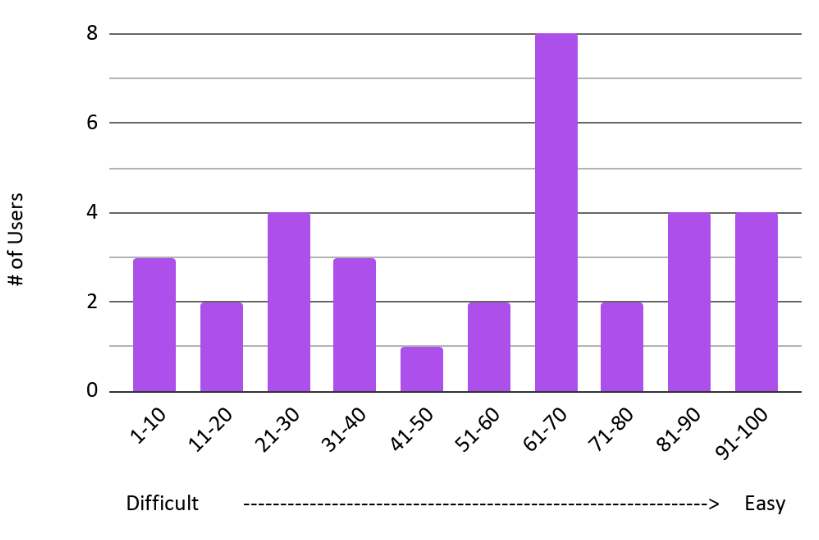
\includegraphics[width=1.0\textwidth]{f1}
\caption[Rating of Summary on Homepage. ]{Rating of Summary on Homepage. \footnotemark.}
\end{figure}
As evident from the graph, there was a wide range of responses. The average user rating of the website was 55. 55 is quite a low value for understanding what Green Drinks is. This supports the results found in the heuristic evaluation. The summary is too long for the average user to understand. The Wix Team [8] suggests that a homepage must be clear and concise. Clear and concise is not what users experience with the current homepage.





\section{Organization and Navigation}
\subsection{Heuristic Evaluation}
Information is the lifeblood of any business or organisation[12]. Hence there is no alternative for the right information at the right place in the world of business, where every industry revolves around the "Internet of Things." The best practices for proper organization and navigation can be put into two  main groups:
\begin{itemize}
\item Information Architecture.
\item Interface Design and Navigation
\end{itemize}

\subsection*{Information Architecture} 
Information Architecture mainly focuses on organizing, structuring, and labelling content in an effective way. In brief, it is something that guides you in a new place. Lynch and Horton[2, chapter 3] say the following are the basic steps in organizing your information:
\subsubsection*{Manage your Inventory}
Inventory is the list of all contents in your website.  Usually, it is also seen as the header buttons on a website that let you go to different pages. The first thing you will notice on the GreenDrinks website is the list of countries they operate.  However, there are no details on what they do and how they do it. Moreover, there is no tagline and the importance of a tagline can be seen at [13]. 

\subsubsection*{Establish a Hierarchical Outline}
Hierarchical organization is a virtual necessity on the web[2, chapter 3]. Design a website as the users see the broadest overview on the first page and move down through the submenus and content pages.  A hierarchical outline is not seen in the GreenDrinks website. Unnecessary information regardless of their priority is shown on the homepage. The information must be put according to their relevance to the users.
 \subsubsection*{Chunk your Information}
Most information on the World Wide Web is gathered in short documents that are intended to be read in a non sequential manner[2, chapter 4]. Chunking allows to organize and present the information in a modular layout that is consistent throughout the website.  This also allows the user to predict the organization of information from his previous page experience. 

Chunking is not done on the GreenDrinks website.  Figure 2 shows how fully packed is the homepage. The homepage is fully stacked up with the list of countries, a video without a caption, and a big paragraph describing the organisation.


%f2 
\begin{figure}[ht]
\centering
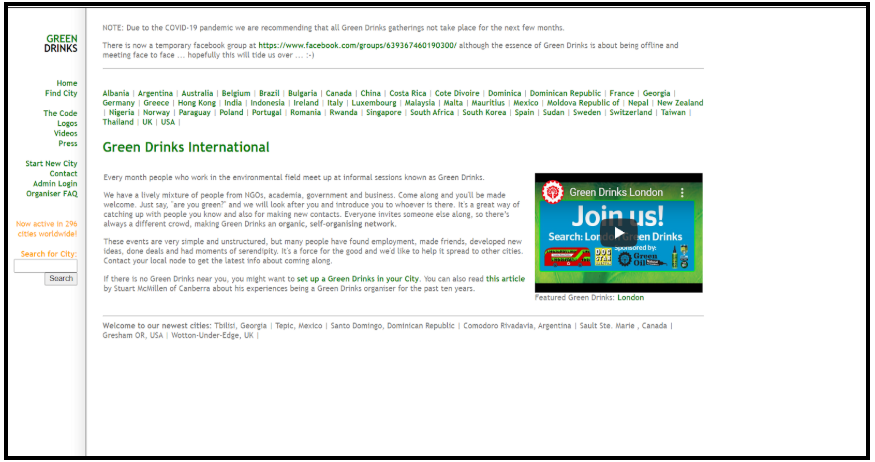
\includegraphics[width=1.0\textwidth]{f2}
\caption[Stacked up Homepage]{Stacked up Homepage. From: http://www.greendrinks.org/\footnotemark.}
\end{figure}

Figure 2: Stacked up Homepage. From: http://www.greendrinks.org/

Stacking them on the homepage is so inconvenient and it makes the website appear to be deviated from showing other essential details[2, chapter 4].

 \subsubsection*{Maintain a Site Structure}
Site structure plays an imperative role in both SEO and usability.  Logically grouping webpages using common folders make it easier for the visitors to move around your site. Site structure reminds about how the website should be arranged.  Moreover, to make your website available to Google, you have to provide the sitemap for proper indexing and crawling. See more information on indexing and crawling at [14].

A logical and consistently named site organization allows users to make successful predictions about where to find things. However, the site structure of  GreenDrinks website is very complicated to form a mental map by the user. The GreenDrinks website is also poorly organized. The header buttons ‘The Code’ and ‘Start New City’ land on the same page, thus clearly failing the test of information architecture practices.

\subsection*{Interface Design and Navigation}
User interface design(UI) is the visual layout of the elements that users might interact within a website.  UI dramatically affects the usability and user experience of an application.  If UI design is too complex or not adapted to targeted users, they may not be able to find the information or the service they are looking for[15]. The following are some of the best  interface design practices from [2] : 

\subsubsection*{Navigating with Right or Left Columns}	
Always be consistent with the layout on all pages. Header navigation is more common these days on the homepage. But moving towards the subpages, Left navigation is more common and people are more used to it[2, chapter 3]. Right navigation is usually used for advertisements, so it can be avoided by the users. 

The GreenDrinks website has used the left column as the navigation bar starting from the homepage to all pages. This is not a big problem but does not meet the 2020 standards. Refer to figure 3 to see a huge area of whitespace on the right side and the bottom due to the left navigation bar.

\begin{figure}[ht]
\centering
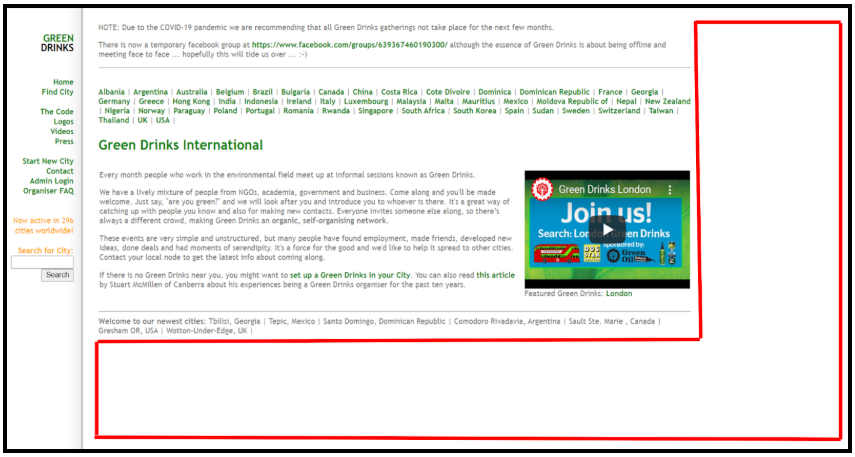
\includegraphics[width=1.0\textwidth]{f3}
\caption[Whitespaces on the Right and Bottom.]{Whitespaces on the Right and Bottom. From: http://www.greendrinks.org/\footnotemark.}
\end{figure}
 
	
The figure shows that the website is also unoptimised for modern browsers. In order to fix these whitespace issues, websites use a header and centered layout.

\subsubsection*{Navigating with Breadcrumb Trails}	
Breadcrumb trails show the structure of a website. These trails start in the home page and end in the major navigation page closest to your current location[2, chapter 4]. Along with the navigation, Breadcrumb trails also allow the users to go back to any page they wish. Please see figure 4 to learn how to use the breadcrumb trails.

\begin{figure}[ht]
\centering
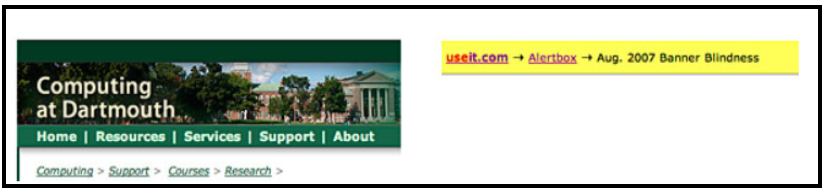
\includegraphics[width=1.0\textwidth]{f4}
\caption[Examples of Breadcrumb Trails]{Two Examples of Breadcrumb Trails Within or Under the Page Header. 
From:  https://webstyleguide.com/wsg3/4-interface-design/3-interface-design.html\footnotemark.}
\end{figure} 

Figure 4 is a perfect example of how to use the Breadcrumb trails. The picture on the left from Computing at Dartmouth has the Breadcrumb trails beneath the menu bar. We can easily understand that the user is in the Research page right now. Similarly, on the right, the useit.com website has the user in the Aug. 2007 Banner Blindness webpage.

Breadcrumb trails are not used on the GreenDrinks website. The home button is available on every page making it easier to return to home. However, there is no feature to go back to the previous page.

The User Interface(UI) is a key component in improving the usability of the website. The UI of the GreenDrinks website is not up to the 2020 standards.  Today, with so many websites being built with WordPress (https://wordpress.com/) and GoDaddy (https://ca.godaddy.com/), the website standard aesthetic increased.  The displays on the site should be formatted in a way that is intuitive for the user to find what they need.  An unmaintained looking website expresses that a company is unmaintained.


\subsection{Survey Results}
For us to get a better understanding of how well Green Drinks organized their information we put an organization question on the survey. The question asked users to rate the organization of the content page of the Green Drinks site. Below in Figure 5 you can find the results of the survey.

\begin{figure}[ht]
\centering
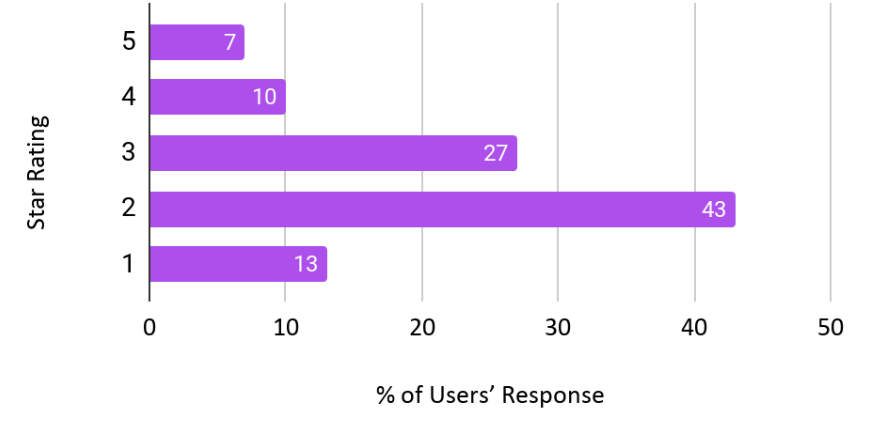
\includegraphics[width=1.0\textwidth]{f5}
\caption[Rating for Organization of Contacts Page]{Rating for Organization of Contacts Page\footnotemark.}
\end{figure} 
The average rating users gave was 2.5 stars out of 5. This result is quite poor. A low rating supports our heuristic findings. A low rating supports that users have a difficult time interpreting the information, navigating the site and understanding the structure. Poor organization of a page can slow users in finding the information they need [15].

\section{Page Layout and Design}



\subsection{Heuristic Evaluation}
Put simply, a web page layout refers to the framework of a site. The aim of any layout is to effectively structure, categorise and present the information a website houses, which in turn shines a light on the most important content and the best journeys for users [16]. Overall, the web page design should provide simple paths for navigation and clearly present information to both the search engines and site users. 
\subsection*{Page Layout }
The page layout is important for a website. The internal pages should have the same layout; secondary pages should be the same as each other, and similar to the internal pages. The  elements that make up the pages on the website include the following:
\begin{itemize}
\item Page Headers
\item Scan Columns
\item Content Areas
\item Page Footers
\end{itemize}

\subsubsection*{Pager Headers}
Web page headers convey the site identity, provide major navigation links, and often offer a search box. The header is where people expect to see a consistent statement of your organizational identity, and the header graphics and text are probably the most important elements in making a collection of web pages feel like an identifiable “site” rather than a random assemblage of files[2, chapter 3].

Instead of using a header area, the GreenDrinks website uses a left navigation bar on all pages. Please see figure 6 to check how crowded the GreenDrinks header area.
\begin{figure}[ht]
\centering
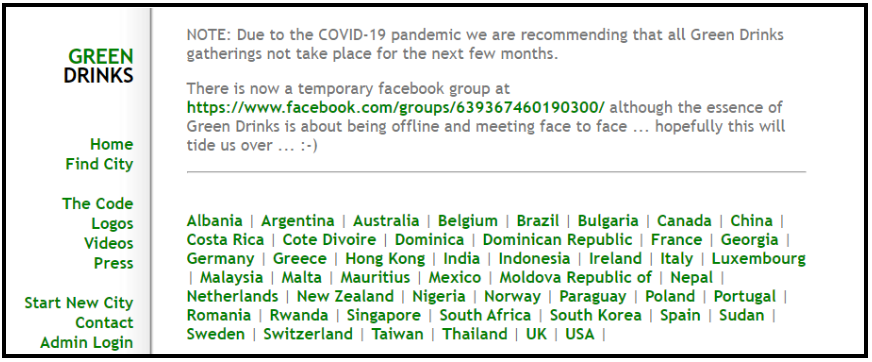
\includegraphics[width=1.0\textwidth]{f6}
\caption[No Header in the Green Drinks Website.]{No Header in the Green Drinks Website.  From: http://www.greendrinks.org/e\footnotemark.}
\end{figure}
 
Page headers are absent on all pages of the GreenDrinks website. There is a logo—which acts as a home button—and a search bar, but they are placed in the scan column because there is no header.
\subsubsection*{Scan Columns}	
Scan columns are usually located on the left side of the page. Important or general navigation links are located here. This makes navigation of websites easier and more user-friendly. Also, the scan column shows how to contact the company of the website[2].

The GreenDrinks website has a scan bar with links to every page of the website. This makes the website easy to navigate. The scan column is missing a way to contact Green Drinks, as there is no phone number or email. Instead of this information being at the bottom of the scan column, it is on its own page of the website.
\subsubsection*{Content Areas}	
Every page needs a title to let the user know the page content. A breadcrumb navigation trail allows the user to keep track and be aware of where documents are located within the website. Navigation links such as jump-to-top, previous page, and next page can also be included in the content area [2].

GreenDrink webpages are well titled, with a main title and many subtitles. There is no breadcrumb navigation trail to inform the user know which link they pressed in the scan column; however, at the very top of the page, the name of the link is stated, but not for all pages. There are no jump-to-top, previous page, or next page links on any of the web pages.

\subsubsection*{Page Footers}	
Page footers are placed at the bottom of the page. They show the author, or the group of people responsible for writing the page, a copyright statement, and contact details. There may also be links to related sites, or more navigation links [2].

Footers are missing in the GreenDrinks website, so there are no navigation links, and the authors’ names are placed somewhere else, if even named. There is no copyright statement on any page, and the contact list is on a web page by itself.
\subsection*{Design Elements}	
There are many elements that contribute to the design of the website. A website’s visual design should be clear and simple, defining functional regions and group-related elements with a visual-hierarchy. This must be done consistently, throughout the website. Pages can be contrasted with graphics and colours [2].
 
Graphics can be illustrations to show, rather than tell; diagrams or charts can be used to show data or results; or, graphics can be a combination of pictures and words [2]. Contrast in colour must be done carefully as some combinations make reading difficult, but if done correctly, the page will stand out. 

Although contrast is good, it can be overdone, so it must be simple and clear. Each page should have a little whitespace around it, so every computer can view the entire page [2].

There is some contrast in the GreenDrinks webpages, but only titles and links are coloured. There is only one graphic on the website, on the home page, a seven-minute video explaining Green Drinks. Though the website has whitespace, there is too much, so there is a lot of unused and empty space.
Survey Results
\subsection{Survey Results}
We placed a question on the survey asking if the user had a good overall graphic experience. This question was based on the entirety of the website, not limited to a single page. Below are the results in Figure 7.

\begin{figure}[ht]
\centering
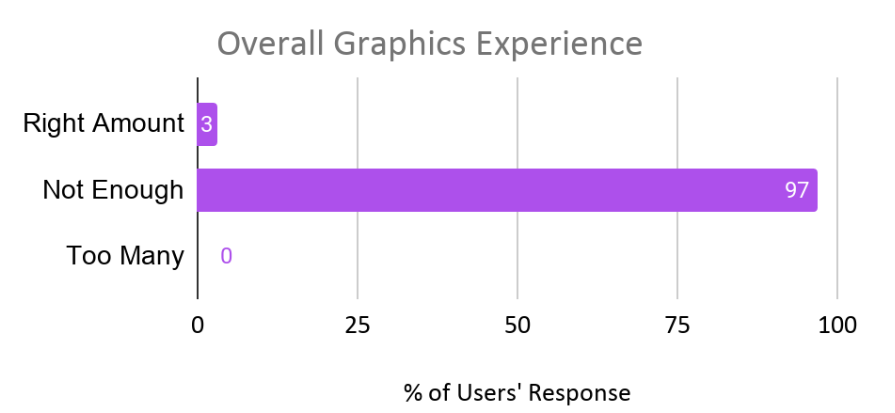
\includegraphics[width=1.0\textwidth]{f7}
\caption[Overall Graphics Experience of the Website.]{Overall Graphics Experience of the Website.\footnotemark.}
\end{figure}

The results are overwhelmingly in the favor of not enough graphics. This is a result of Green Drinks heavily favoring using text to explain rather than images.This supports findings in the heuristic report. In order for a website to be successful in it’s design graphics are needed to show not tell the user[2]. Graphics give a pleasant variation in the information presented.

\section{Content and Interactive Features}
\subsection{Heuristic Evaluation}
Websites designers take many practices to improve their usability. These practices enable users to maneuver the website with ease, allow individuals to pick up information easier, understand the content of the website, and allow individuals with disabilities to use the website. The criteria used for evaluation are the following:
\begin{itemize}
\item Interactive Features
\item Available and Accessible
\item	Scannable Content
\item	Usable for Impaired
\end{itemize}


\subsection*{Interactive Features}
People prefer websites with interactive features, good web interface and links that can lead to other pages. The Nielsen Norman Group [17] did a study on what individuals desire in a website and how they viewed certain websites. Throughout the study, most individuals reported that they disliked websites that were simply just blocks of tests. 

People expect a more graphical and interactive level from websites. It creates a more usable website, while keeping the users engaged. For social purposes, people want a website that allows online interaction with other users of the site. Thus, it is recommended to create chat boxes, and forums for website users.

The Green Drinks website heavily lacks interactive features on its website. It has only 1 video on the home screen and a search bar for the city. The website consists only of paragraphs, and blocky texts. Some pages are blank and do not have anything on them. The website also lacks any forums or chat boxes, despite being a website for social gatherings.

\subsection*{Availability and Accessibility}
People want a website that is readily available and accessible. One way of making a website more usable is to have a good search engine. A good search engine makes it so that individuals do not have to go scrolling through the website, but instead type in what they wanted to be directed to. 

A survey response from the Nielsen Norman Group research case said, ‘A good search engine is key for a good website’ Others stated that they requested a ‘Find command’,  or the ability to search what they want on the website [17, Study 1: Directed Tasks, Findings, para. 1]. Another solution is to maintain server uptime. This means that the website is always online and rarely under maintenance.

For the most part, the GreenDrinks website is accessible to the public. The website does not consist of many memory heavy interactions, making it easy to load. The website server is rarely offline, meaning the server is mostly online and accessible to frequent users. There is a ‘Search for Cities’ search bar, making it easy for users to look for their city.

\subsection*{Scannable Information}
When people maneuver a website, they want to get the information as fast as possible. According to Quicksprout [18], “55\% of people spend less than 15 seconds actively on a website.” [18, What you’re up against, para. 2]. Quicksprout also states that less than 79\% of people read word-by-word [18, What you’re up against, para. 5]. Therefore, content created for websites should be designed to be scannable. 

Websites create scannable information through these methods: writing shorter paragraphs, keeping short sentences, following the “four-syllable rule”, using sub headers, using images, adding links, using bullet points, and creating lists[18]. These strategies allow readers to scan the information quickly, so they do not have to spend much time on the website.

The Green Drinks website is not very scannable, as it consists mainly of wordy, blocky paragraphs of text. There are no bolded or highlighted texts, making it difficult for the reader to pick out important information. It does not consist of any images, which may bore the readers. However, pages do consist of subheadings, making it easy for users to determine what the paragraph will be talking about.

\subsection*{Usability for the Impaired}
Scrolling through websites is challenging for individuals with visual disabilities. Text too small is difficult for readers with visual impairments. In other cases, the pictures are not visible for certain people.

A solution to this is a magnifying tool [19, What are the most popular types of assistive technology for using the internet, List 1] . The tool allows the reader to zoom in to specific texts or parts of the screen. This allows readers with visual impairments the ability to read the website with much ease. The optics for the magnifying glass can be adjusted to the reader’s choice, making it more comfortable for them. Another solution is the use of automated readers [19, What are the most popular types of assistive technology for using the internet, List 1]. 

Readers with visual impairments such as dyslexia, magnification may not be a suitable solution. Websites introduce the opportunity for text-to-speech readers, which gets an automated reader to read what is on the screen.

The GreenDrinks website mainly consists of texts and writing. There is no way for a reader to magnify paragraphs. It makes it more difficult for readers with visual impairments to read the website. There is also no reader for the website, which also creates difficulty for those with visual impairments to read through the website.



\subsection{Survey Results}
To test if the page was scannable we asked users what they first saw on the homepage. Quicksprout [18] says that scannability is important so that users actually read the content. Below are the results of the survey in Figure 8.
\begin{figure}[ht]
\centering
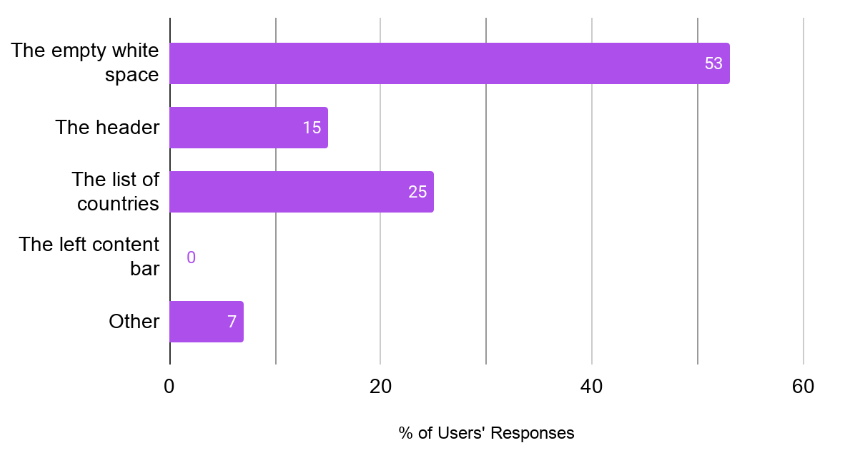
\includegraphics[width=1.0\textwidth]{f8}
\caption[What is First Noticed on the Homepage.]{What is First Noticed on the Homepage.\footnotemark.}
\end{figure}

Figure 8: What is First Noticed on the Homepage.

As evident from the survey, the white space is the most looked at item. 25 percent of people did look at the list of countries which is one of the main goals of the homepage, but 53\% were distracted by the whitespace. The survey results once again support our heuristic findings. The site doesn’t make the summary short enough for it to catch users’ eyes. Additionally, the whitespace in its current state is counterproductive.

\section{Conclusions}
The purpose of this study was to determine the overall organization, strategy and style of the Green Drinks website. These aspects are important in a website because they allow the readers to attain the required information, keep users interested, and understand the goals of the website.

\subsection*{Style}
At first sight, we believed that there was no clear strategy for the Green Drinks website. We were unable to determine the organization's goals and objectives. Additionally, there is no proper framework or lacks direction to important information. The website’s layout is very confusing and lacks interaction, making the site hard to use. If the website includes a clear goal or mission statement in the home page, then this would solve an issue with its strategy. It is also beneficial if the website makes it easier to organize meetups and gatherings on the website. 
\subsection*{Organization}
The organization of the Green Drinks website did not meet our expectations. Every page on the website consists of text and paragraphs. The information is not scannable or concise, making it very difficult for the readers to understand the context. Readers would have to spend an extended amount of time reading the website to understand the information. This could be resolved through bolding and highlighting important words throughout the page. The information should be compacted so the information is more scannable. 
\subsection*{Strategy}
The visuals of this website were lower than standard, and did not meet the groups expectations. The website consists mainly of paragraphs and text, which many readers claim to dislike. Additionally, there were no pictures or visuals. These aspects make the website very boring, and unmotivating to read. It also leads to difficulty for the visually impaired to read. This could be solved through reducing the paragraph size and increasing the fonts. Another solution would be to include graphics to create a visually appealing website.
\section{Recommendations }
\subsection*{Reduce the size of paragraphs to be more scannable}
The Green Drinks website mainly consists of paragraphs and text. This makes the website difficult to read. The website should reduce the size of its paragraphs and text. This would make the website more interesting and readable for its viewers. It also allows for more scannable information so that readers can gather the information they need quicker.


\subsection*{Make the website more visually appealing}
At first glance, the website’s aesthetics are unappealing. Most of the survey results reported that there were no graphics on the website, and that they dislike the blank white space on certain pages. This can be resolved by integrating visuals and graphics into the pages. Lastly, the list of cities at the top of the website should be removed. This will make the website more visually appealing, and create a good impression for the readers.


\subsection*{Reformat the homepage to guide users to Find City}
The website has three different ways to find a designated city. This is redundant since all three options lead to the same place. One of these options leads to a list of cities, which makes it difficult for readers to find their desired city. This can be improved by replacing the current ‘Find City’ functions with a Find City button. Additionally, the page of cities at the top of the page should be removed. This will make it easier for viewers to find their city and remove redundancies.


\subsection*{Add important information to homepage}
When viewers first visit the website, there is no clear objective or mission statement. This will often confuse viewers because it will be unclear what the purpose of the website is. One solution would be to include a tag line of the organization, or a summary of your goals. Doing this will tell your viewers the purpose of the website. \skiplines{4}



\begin{center}

\ding{91}  \ding{91} \ding{91} \ding{91}

\end{center}


\pagebreak

\section{References}

\begin{thebibliography}{9}

\bibitem{greendrinkswebsite}
E. Datschefski, P. Scott, I. Grant, and Y. Benjamin, Green Drinks. [Online]. Available:	\\\texttt{http://www.greendrinks.org} [Accessed: June 16, 2020].

\bibitem{lynch}	
P. J. Lynch and S. Horton, “Web Style Guide (3rd edition),” 2009. [Online]. Available: \\\texttt {https://webstyleguide.com/wsg3/index.html}[Accessed: June 16, 2020].

\bibitem{Ewald}
T. Ewald,\textit{ Writing in the Technical Fields: A Practical Guide}, 2nd ed. pp. 242 Oxford University Press., 2017. 


\bibitem{rules}
 "10 Rules of Web Design," \textit{Sharpened}, 12-Dec-2019. [Online]. Available: \\\texttt{https://sharpened.com/web\_ design\_ rules}. [Accessed: June 16, 2020]. 
 
 
\bibitem{design}
"Designing Multiple-Choice Questions," Centre for Teaching Excellence, 27-Jun-2017. [Online]. Available: https://uwaterloo.ca/centre-for-teaching-excellence/teaching-resources/teaching-tips/developing-assignments/assignment-design/designing-multiple-choice-questions [Accessed: June 16, 2020].


 \bibitem{lk}
 L. K. Lawless, “Yes / No questions (closed questions),” \textit{Lawless English}, 18-Apr-2014. [Online]. Available: \\\texttt{https://www.lawlessenglish.com/learn-english/grammar/questions-yes-no/} [Accessed: June 16, 2020].
 
 \bibitem{sf}
 S. Farrel, “Open-Ended vs. Closed-Ended Questions in User Research,” \textit{Nielsen Norman Group}. [Online]. Available: \\\texttt{https://www.nngroup.com/articles/open-ended-questions/}. [Accessed: June 16, 2020].
 
 \bibitem{wix}
The Wix Team, “How To Build A Killer Homepage - 10 Tips,” \textit{Wix Blog}, 24-Jul-2019.
[Online]. Available:
\\\texttt{https://www.wix.com/blog/2014/01/build-a-killer-homepage-10-dos-donts}.
[Accessed: June 16, 2020].

\bibitem{g}
G. Benedict, “How to Boost Conversion Rate with Web Design?,” \textit{Hacker Noon}, 
Jun-2020. [Online]. Available: 
\\\texttt{https://hackernoon.com/how-to-boost-conversion-rate-with-web-design-cc8faa7b
829d}. [Accessed: June 16, 2020].
	
\bibitem{khicks}
K. Hicks, “How To Make A Website Mobile Friendly,” \textit{HostGator Blog}, 28-Feb-2020.
[Online]. Available:
\\\texttt{https://www.hostgator.com/blog/how-make-website-mobile-friendly/}. [Accessed: June 16, 2020].

\bibitem{bclay}
B. Clay, “7 Mobile-Friendly Navigation Best Practices,” \textit{Bruce Clay, Inc.},    22-Jul-2019. 
[Online]. Available: \\\texttt{https://www.bruceclay.com/blog/mobile-friendly-navigation/}
[Accessed: June 16, 2020].

\bibitem{how}
 “How Important is Information Management ?,”  \textit{Edology}, Available: \\\texttt{https://www.edology.com/blog/computing-it/how-important-is-information-management/} [Accessed: June 16, 2020].

\bibitem{vgendelman}
 V. Gendelman,  “Why Your Company Needs A (Good) Tagline,”  \textit{Forbes}, Available: \\\texttt{https://www.forbes.com/sites/theyec/2014/11/03/why-your-company-needs-a-good-tagline/\#25b49746d5be} [Accessed: June 16, 2020].

\bibitem{seo}	
“The Beginner’s Guide to SEO,” \textit{Moz Pro}, Available: \\\texttt{https://moz.com/beginners-guide-to-seo/how-search-engines-operate} [Accessed: June 16, 2020].	

\bibitem{uid}
 “User Interface Design,” \textit{Pidoco}, Available:\\\texttt{https://pidoco.com/en/help/ux/user-interface-design} [Accessed: June 16, 2020].


\bibitem{hdaly}
H. Daly, “Why design and layout are important for all web pages,” \textit{The Telegraph UK}, November 29, 2019. [Online] Available: \\\texttt{https://www.telegraph.co.uk/branded-content/marketing-guides/why-web-page-design-important/} [Accessed: June 16, 2020].


\bibitem{jniel}
J. Nielsen and J. Morkes,”Concise, SCANNABLE, and Objective: How to Write for the Web,” \textit{Nielsen Norman Group Concise}. [Online]. Available: \\\texttt{https://www.nngroup.com/articles/concise-scannable-and-objective-how-to-write-for-the-web/} [Accessed: June 16, 2020].

\bibitem{tstep}
“The Step-by-Step Guide to Creating Scannable Content,” \textit{Quick Sprout}. [Online]. Available: \\\texttt{https://www.quicksprout.com/the-step-by-step-guide-to-creating-scannable-content/} [Accessed: June 16, 2020].

\bibitem{cratcliff}
C. Ratcliff, “How to design websites for blind and partially sighted people,” \textit{Userzoom/Betterux}. [Online]. Available: \\\texttt{ https://www.userzoom.com/blog/how-to-design-websites-for-blind-and-partially-sighted-people/}. [Accessed: June 16, 2020].

	
	
\end{thebibliography}

\newpage \section{Appendices}
\subsection*{Appendix A: Individual Heuristic Reports}
This appendix will show how we divided the website analysis between the four team members and initial analysis findings. Each member wrote their individual heuristic reports on these assigned sections.

\subsubsection*{1. Overview \& Universal Usability - Jade Fjestad}

Initial Findings:
\begin{itemize}
\item Set clear goals for the website, then create a project charter document to be the blueprint of the site
really communicate the 3 most important ideas
\item Know your audience 
\item Use Web analytics to get data about your user
\item Design critiques, try to start with many ideas then work towards the best one
\item Content inventory, tends to be the weakest link of the website be sure it’s done early and done well
\item Stay away from visual design until everything else is planned
\item Simple is good

\item Make accessible to disabled people Web Accessibility Initiative (WAI) has guidelines, universal design (usable by everyone ex. ramp)
\item Use user centered design (UCD) ask the user what they want from the site
\item Design process, user research 
\end{itemize}

\subsubsection*{2. Organization of information \& navigation tools and links - Tomin Mattam}
Initial Findings:
\begin{itemize}
\item Organize the site content into taxonomies and hierarchies of information.
\item Research and design the core site navigation concepts.
\item Establish a hierarchical outline of your content and create a controlled vocabulary so the major content, site structure, and navigation elements are always identified consistently.
\item List of countries at top – problem, should be with a title and what they do at these countries.
\item No information about what they do 
\item No tagline 
\item No clue about organization
\item Orientation: Where am I am right now
\item Very hard to find the route to go 
\item When the person come back, he will only have a very short idea about how the website works 
\item Must have a link to come back to home screen all the time 

\item It will be better to have the bar on the top than on left side 
\item No clear info about date and time of the activities happening in the organization.
\end{itemize}

\subsubsection*{3. Page layout, design elements, typography, headings, \& visuals - Jonathan Ballarin}
Initial Findings:
\begin{itemize}
\item Page Headers are at top of each page that include tools and the search bar
\item Content area includes a title page, a breadcrumb trail, jump to top links and previous and next page links
\item Page footer includes the author or whatever group is responsible, a copyright statement, the date the page was published, and contact details
\item Consistent design on pages
\item Contrast but keep it simple
\item Role of web graphics
\item Pages have a hierarchy or are tiered
\item All initial pages are the same layout, and all secondary pages have the same layout, but secondary pages are slightly different than initial pages
\item Home page includes an identity for the site and company, a clear focus and goals, and tools
\end{itemize}

\subsubsection*{4. Content (clarity, helpfulness) \& usability of interactive features (e.g., membership forms, contact links) - Curtis Eck}
Initial Findings:
\begin{itemize}
\item Readers are not just looking at one site, but rather many others. It is easier for them to set up links and other ways to access information on the site
\item Authors tend to use hypertext links as a form of context. Making it easier for individuals to access the citation.
\item When on a website, people despise downloading/waiting for their information
\item With no sustain in narrative, people are sent to search for information
\item Although some authors use hyperlink, people are beginning to move away from them
\item There has been an increase in demand for more interactive websites
\item Website creators are beginning to create more interactive websites
\item As of recently, many users expect sophisticated and interactive websites
\item Most users tend to scorn/dislike the text based simple styled websites
\item People desire a good search engine on the website
\end{itemize}

 

\newpage
\subsection*{Appendix B: Web Based Survey}
The survey was sent out to the COMS 363 and consists of 9 questions to evaluate both the usability parameters and user experience. All the survey responses remained private and only the data will be extracted out. The survey was designed at best effort to keep it short and easier for the respondent.

Thank you for taking our survey! We’d like to ask you about your impressions of our website \\\texttt{http://www.greendrinks.org/} to help us better serve you. In return, I will be happy to do your survey. Send it to me. 

\textit{The survey that will be sent out to the COMS 363 will consist of questions to evaluate both the usability parameters and user experience. All the survey responses will remain private and only the data will be extracted out. The survey is designed at best effort to keep it short and easier for the respondent. See below:
This anonymous survey is being conducted as part of a student project in Coms 363, a course in Professional and Technical Communication at the University of Calgary. This survey is being administered via SurveyMonkey, an online survey tool that does not track respondents’ names or e-mail information. No names will be connected with any of the responses collected. By completing and submitting this survey, you are indicating your informed consent to participate in this research project. You may withdraw at any time while completing the survey simply by exiting the survey. Since results are not tracked, you cannot withdraw your participation once you hit submit. If you have any questions about this survey, please contact my instructor, Andrea Hanslip (email: arhansli@ucalgary.ca). Thank you.}

\begin{itemize}
\item[1] How visually appealing is our Homepage?
\subitem Extremely appealing
\subitem Very appealing
\subitem Somewhat appealing
\subitem Not so appealing
\subitem Not at all appealing

\item[2] What did you first notice on the home page?
\subitem The empty whitespace
\subitem The header “Green Drinks International” and text that talks about Green Drinks
\subitem  The list of countries
\subitem The left content bar
\subitem Other (please specify)


\item[3] How easy is it to find out what Green Drinks is about?
\subitem 1(No clue)
\subitem Hardly
\subitem 5(Yeah!)

\item[4] Was it easy to find your city?
\subitem Very hard
\subitem Hard
\subitem Neither
\subitem Easy 
\subitem Very Easy 

\item[5] Do you agree “Layout of the pages made the performance of tasks very difficult”?
\subitem 0(Disagree)
\subitem Ok
\subitem 5(Agree)

\item[6] Play the video on the “Home” page.
\subitem Is the length of the video too long
\subitem Is the length of the video just right
\subitem Is the length of the video too short

\item[7] Go to the “Contact” page and rate the organization of the page.
\subitem* (Rated out of 5 stars)

\item[8] How is the overall graphics experience?
\subitem Too Many 
\subitem Not enough
\subitem Right Amount

\item[9]  Comment on your overall impression of the Green Drinks website.
\subitem* (open ended)
\end{itemize}

\end{document}